\documentclass[11pt,aspectratio=169]{beamer}
\usepackage[utf8]{inputenc}
\usepackage[T1]{fontenc}
\usepackage{amsmath}
\usepackage{amsfonts}
\usepackage{amssymb}
\usepackage{graphicx}
\usepackage{tikz}
\usepackage{booktabs}
\usepackage{color}
\usetheme{metropolis}   

% images
\graphicspath{ {D:/Users/saketh/Documents/GitHub/BECCS-Case-Study/} }

% sig stars
\def\sym#1{\ifmmode^{#1}\else\(^{#1}\)\fi}

\author{Saketh Aleti}
\title{Estimation of CGE Parameters}
%\subtitle{}
%\logo{}
%\institute{}
\date{\today}
%\subject{}
%\setbeamercovered{transparent}
%\setbeamertemplate{navigation symbols}{}



\begin{document}
	
	
\maketitle

\begin{frame}{Outline}

\begin{itemize}
	\setlength\itemsep{1.5em}
	\item CES vs. CET Theory
	
	\item Fossil Fuel Results
	
	\item Renewables Results
	
\end{itemize}

\end{frame}

\begin{frame}{Theory}

	\metroset{block=fill}
	
	
	\begin{block}{\centering{CES/CET Problem}}
	\large \begin{align*}
	 \\[-3em] \text{\textbf{Prod./Trans. Function}: } &Q = \theta \cdot \left( \sum_i \; \alpha_i \cdot X_i^\phi \right)^{1/\phi} \\[1em]
	\text{\textbf{Budget Constraint}: } &B = \sum_i \;p_i \cdot  X_i \\[-2.5em]
	\end{align*}
	\end{block}
	

	\begin{itemize}
		\item $p_i$ are prices, $\theta$ is the scaling coefficient, $\alpha_i$ is the share coefficient, $B$ is the budget
		\item The elasticity of substitution is $\sigma = 1 / (1-\phi)$
		\item The elasticity of transformation is $\psi = 1 / (\phi - 1)$
	\end{itemize}
\end{frame}




\begin{frame}{CES versus CET - CES Example}

\begin{columns}[T,onlytextwidth]
	\column{0.5\textwidth}
	
	\begin{figure}
		\hspace{-2em}
		\vspace{1em}
		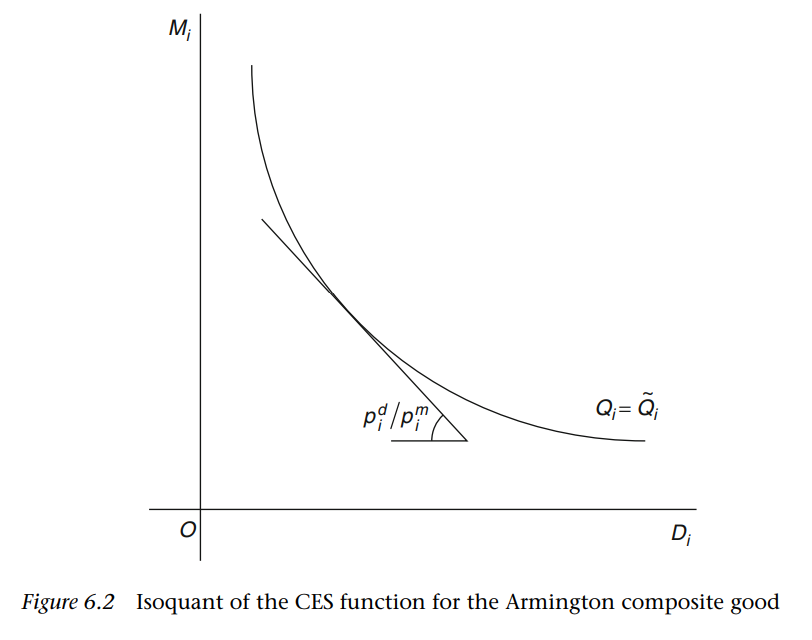
\includegraphics[width=1\textwidth]{exhibits/CES_example.PNG} 
	\end{figure}
	
	\column{0.5\textwidth}
	
	\begin{itemize}
		
		\setlength\itemsep{2em}
		
		\item Isoquant of imported good $M_i$ and domestic good $D_i$ shows combination needed to produce a fixed quantity $\tilde{Q_i}$
		
		\item Consumer wants to satisfy a utility function including the composite $Q_i$ 
		
		\item Convexity shows diminishing returns to consuming only $M_i$ or $D_i$
		
	\end{itemize}
	
\end{columns}

\end{frame}



\begin{frame}{CES versus CET - CET Example}

\begin{columns}[T,onlytextwidth]
	\column{0.5\textwidth}
	
	
	\begin{figure}
		\hspace{-2em}
		\vspace{1em}
		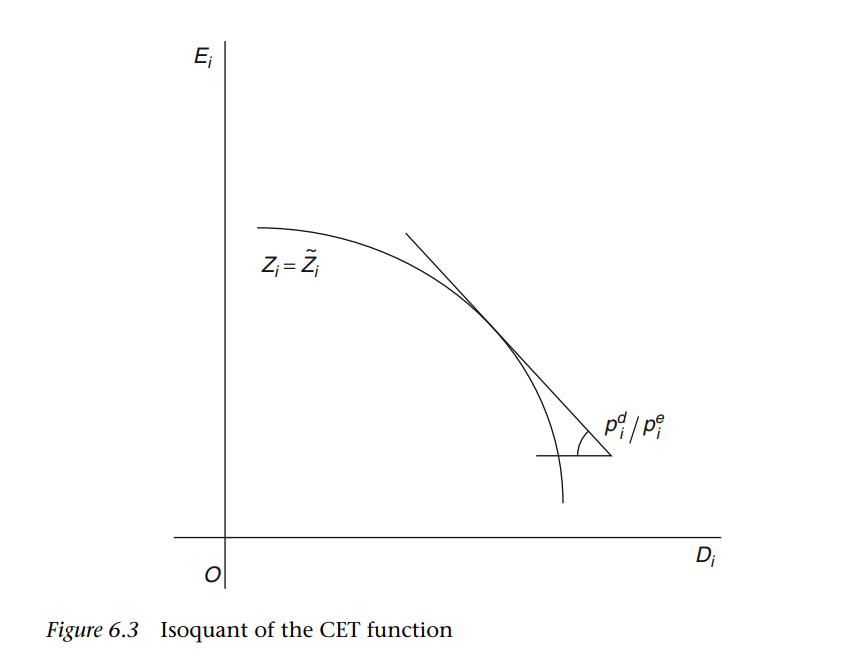
\includegraphics[width=1\textwidth]{exhibits/CET_example.PNG} 
	\end{figure}
	
	\column{0.5\textwidth}
	
	\begin{itemize}
		
		\setlength\itemsep{1.5em}
		
		\item Isoquant of exports $E_i$ and domestic supply $D_i$ of some good $i$
		
		\item Shows combination needed to reach a GDP of $\tilde{Z_i}$
		
		\item Firms maximize profit by selling goods where they are most valued
		
		\item Concavity shows diminishing returns to selling everything domestically versus exporting everything
		
	\end{itemize}
	
\end{columns}

\end{frame}


\begin{frame}{CES/CET Solution}

	\metroset{block=fill}

	\vspace{0.5em}

	\begin{block}{\centering{CES/CET Problem}}
		\large \begin{align*}
		\\[-3em] \text{\textbf{Prod./Trans. Function}: } &Q = \theta \cdot \left( \sum_i \; \alpha_i \cdot X_i^\phi \right)^{1/\phi} \\[1em]
		\text{\textbf{Budget Constraint}: } &B = \sum_i \;p_i \cdot  X_i \\[-2.5em]
		\end{align*}
	\end{block}

	\vspace{-1em}
\
	$$\text{Profit Maximization} \implies \frac{X_i}{X_j} = \left(\frac{\alpha_i \cdot p_j}{\alpha_j \cdot p_i}\right)^{1/(1-\phi)}$$
	
	$$\implies \ln\left(\frac{X_i}{X_j}\right) = \sigma \cdot \ln\left(\frac{\alpha_i \cdot p_j}{\alpha_j \cdot p_i}\right) = \psi \cdot \ln\left(\frac{\alpha_j \cdot p_i}{\alpha_i \cdot p_j}\right) $$

\end{frame}


\begin{frame}{Methodology}

	\metroset{block=fill}
	
	\vspace{0.5em}
	
	\begin{block}{\centering{CES $\implies$ Functional Form}}
	$$\ln\left(\frac{X_{i,s,t}}{X_{j,s,t}}\right) = \sigma \cdot \ln\left(\frac{ p_{j,s,t}}{ p_{i,s,t}}\right) + c_{s,t} + \varepsilon_{s,t}$$
	\end{block}
	
	\vspace{-0em}
	
		\begin{itemize}
			
			%\setlength\itemsep{1.5em}
		
			\item Inputs $i$ and $j$ in state $s$ at time $t$
			
			\item $X_i$ and $X_j$ are the input quantities, $p_i$ and $p_j$ are the input prices
			
			\item Share parameters from previous equation are absorbed into the constant term
			
			\item This approach avoids endogeneity problems since the input ratios are not dependent on any variables except for price $\implies$ demand is fixed, supply movements trace out demand curve
			
		\end{itemize}

\end{frame}




\begin{frame}{Methodology (cont.)}

\metroset{block=fill}

\vspace{0.5em}

\begin{block}{\centering{CES $\implies$ Functional Form}}
	$$\ln\left(\frac{X_{i,s,t}}{X_{j,s,t}}\right) = \sigma \cdot \ln\left(\frac{ p_{j,s,t}}{ p_{i,s,t}}\right) + c_{s,t} + \varepsilon_{s,t}$$
\end{block}

\vspace{-0em}

\begin{itemize}
	
	%\setlength\itemsep{1.5em}
	
	\item Elasticity of substitution/transformation is the same between all commodities in the production/transformation function 
	
	\item Suppose coal ($i$), natural gas ($j$), and oil ($k$) are all part of the same production function for electricity
	\begin{align*}
	\implies &\ln(X_i/X_j) = \, \sigma \ln(p_j / p_i) + c_{1,s,t} + \varepsilon_{1,s,t} \\
	= &\ln(X_j/X_k) = \sigma \ln(p_k / p_j) + c_{2,s,t} + \varepsilon_{2,s,t} \\
	= &\ln(X_i/X_k) = \sigma \ln(p_k / p_i) + c_{3,s,t} + \varepsilon_{3,s,t}
	\end{align*}
	
\end{itemize}

\end{frame}


\begin{frame}{Methodology (cont.)}

\metroset{block=fill}

\vspace{0.5em}

\begin{block}{\centering{CES $\implies$ Functional Form}}
	$$\ln\left(\frac{X_{i,s,t}}{X_{j,s,t}}\right) = \sigma \cdot \ln\left(\frac{ p_{j,s,t}}{ p_{i,s,t}}\right) + c_{s,t} + \varepsilon_{s,t}$$
\end{block}

\vspace{-0em}

\begin{itemize}
	
	%\setlength\itemsep{1.5em}
	
	\item Elasticity of substitution/transformation is the same between all commodities in the production/transformation function 
	\begin{align*}
	\implies &corr(\ln(X_i/X_j), \,\ln(p_j / p_i)) \\
	= &corr(\ln(X_j/X_k), \ln(p_k / p_j)) \\
	= &corr(\ln(X_i/X_k), \ln(p_k / p_i))
	\end{align*}
	
	\item So, regressions are done by regressing all unique pairs with coefficients constrained to be equal 
	
	
\end{itemize}

\end{frame}


\begin{frame}{Methodology (cont.)}

\metroset{block=fill}

\begin{itemize}
	
	\setlength\itemsep{1em}
	
	\item Constrained regressions on $n*(n-1)/2 -1$ sets of equations
	
	\item EG: (Coal/NatGas + Oil/NatGas), (Coal/NatGas + Oil/Coal), (Oil/Coal + Oil/NatGas)
	
	\item Theoretically, any set of equations in parenthesis should give the same results as another set of equations in parenthesis
	
	\item Data comes from the EIA for each state in 2016
	
	\begin{itemize}
		\item Factor input quantities are set to the amount of each used to generate electricity
		
		\item Factor prices are set to the be the average cost of the each input
		
		\item Coal given thousand tons, Natural gas in thousand McF, and oil in thousand barrels
	\end{itemize}
	
\end{itemize}

\end{frame}




\begin{frame}{Fossil Fuel Results}

\fontsize{6pt}{7}\selectfont
\begin{center}
\begin{table}
	\caption{Elasticity of Substitution for Fossil Fuels } 
	\begin{tabular}{@{\extracolsep{0.5em}}lcc|cc|cc} 
		\\[-8ex]\hline  
		\hline \\[-1.2ex]  
		& \multicolumn{6}{c}{\textit{\scriptsize Dependent variable: Difference in Log Inputs}} \\ [0.5em] 
		\cline{2-7}  \\[-0.5em] 
		& ln(Coal/NatGas) & ln(Coal/Oil) & ln(Coal/NatGas) & ln(Oil/NatGas)  & ln(Coal/Oil) & ln(Oil/NatGas) \\ \\ [-0.7em]
		\hline \\[-1.2ex] 
		ln($p_{natgas}/p_{coal}$)&   \colorbox{yellow}{$1.002^{***}$} &  & \colorbox{yellow}{$1.013^{***}$} &  &  &  \\ 
		& $(0.209)$ &  & $(0.210)$ &  &  &  \\ [0.5em]
		ln($p_{oil}/p_{coal}$)&  & $1.002^{***}$  &  &  & \colorbox{yellow}{$1.004^{***}$} &  \\ 
		&  & (0.209) &  &  & $(0.209)$ &  \\ [0.5em]
		ln($p_{natgas}/p_{oil}$)&  &  &  & $1.013^{***}$  &  & $1.004^{***}$ \\ 
		&  &  &  & $(0.210)$ &  & $(0.209)$ \\ [0.5em]
		Constant & $-2.429^{***}$ &  $-1.782^{***}$ & $-2.411^{***}$ & $-0.623$ & $-1.783^{***}$ & $-0.643$  \\ 
		&  $(0.398)$ & $(0.190)$ & $(0.399)$ & $(0.519)$ & $(0.190)$ & $(0.517)$ \\ [0.5em]
		State Dummies & \checkmark & \checkmark & \checkmark & \checkmark & \checkmark & \checkmark \\ \\ [-0.5em]
		\hline \\ [-0.5em] 
		Observations & 109 & 109 & 109 & 109  & 109    & 109  \\ [0.25em]
		R$^2$ & 0.9284  & 0.9399 &  0.9284 &  0.8643 &  0.9399 & 0.8642  \\  [0.25em]
		Chi$^2$ & $1414^{***}$ & $1732^{***}$ & $1427^{***}$ & $706^{***}$ & $1725^{***}$ &  $701^{***}$ \\
		\\ [-0.75em] 
		\hline \hline
	\end{tabular} 
\end{table}

\end{center}

\end{frame}





\begin{frame}{Fossil Fuel Results}

\begin{center}
	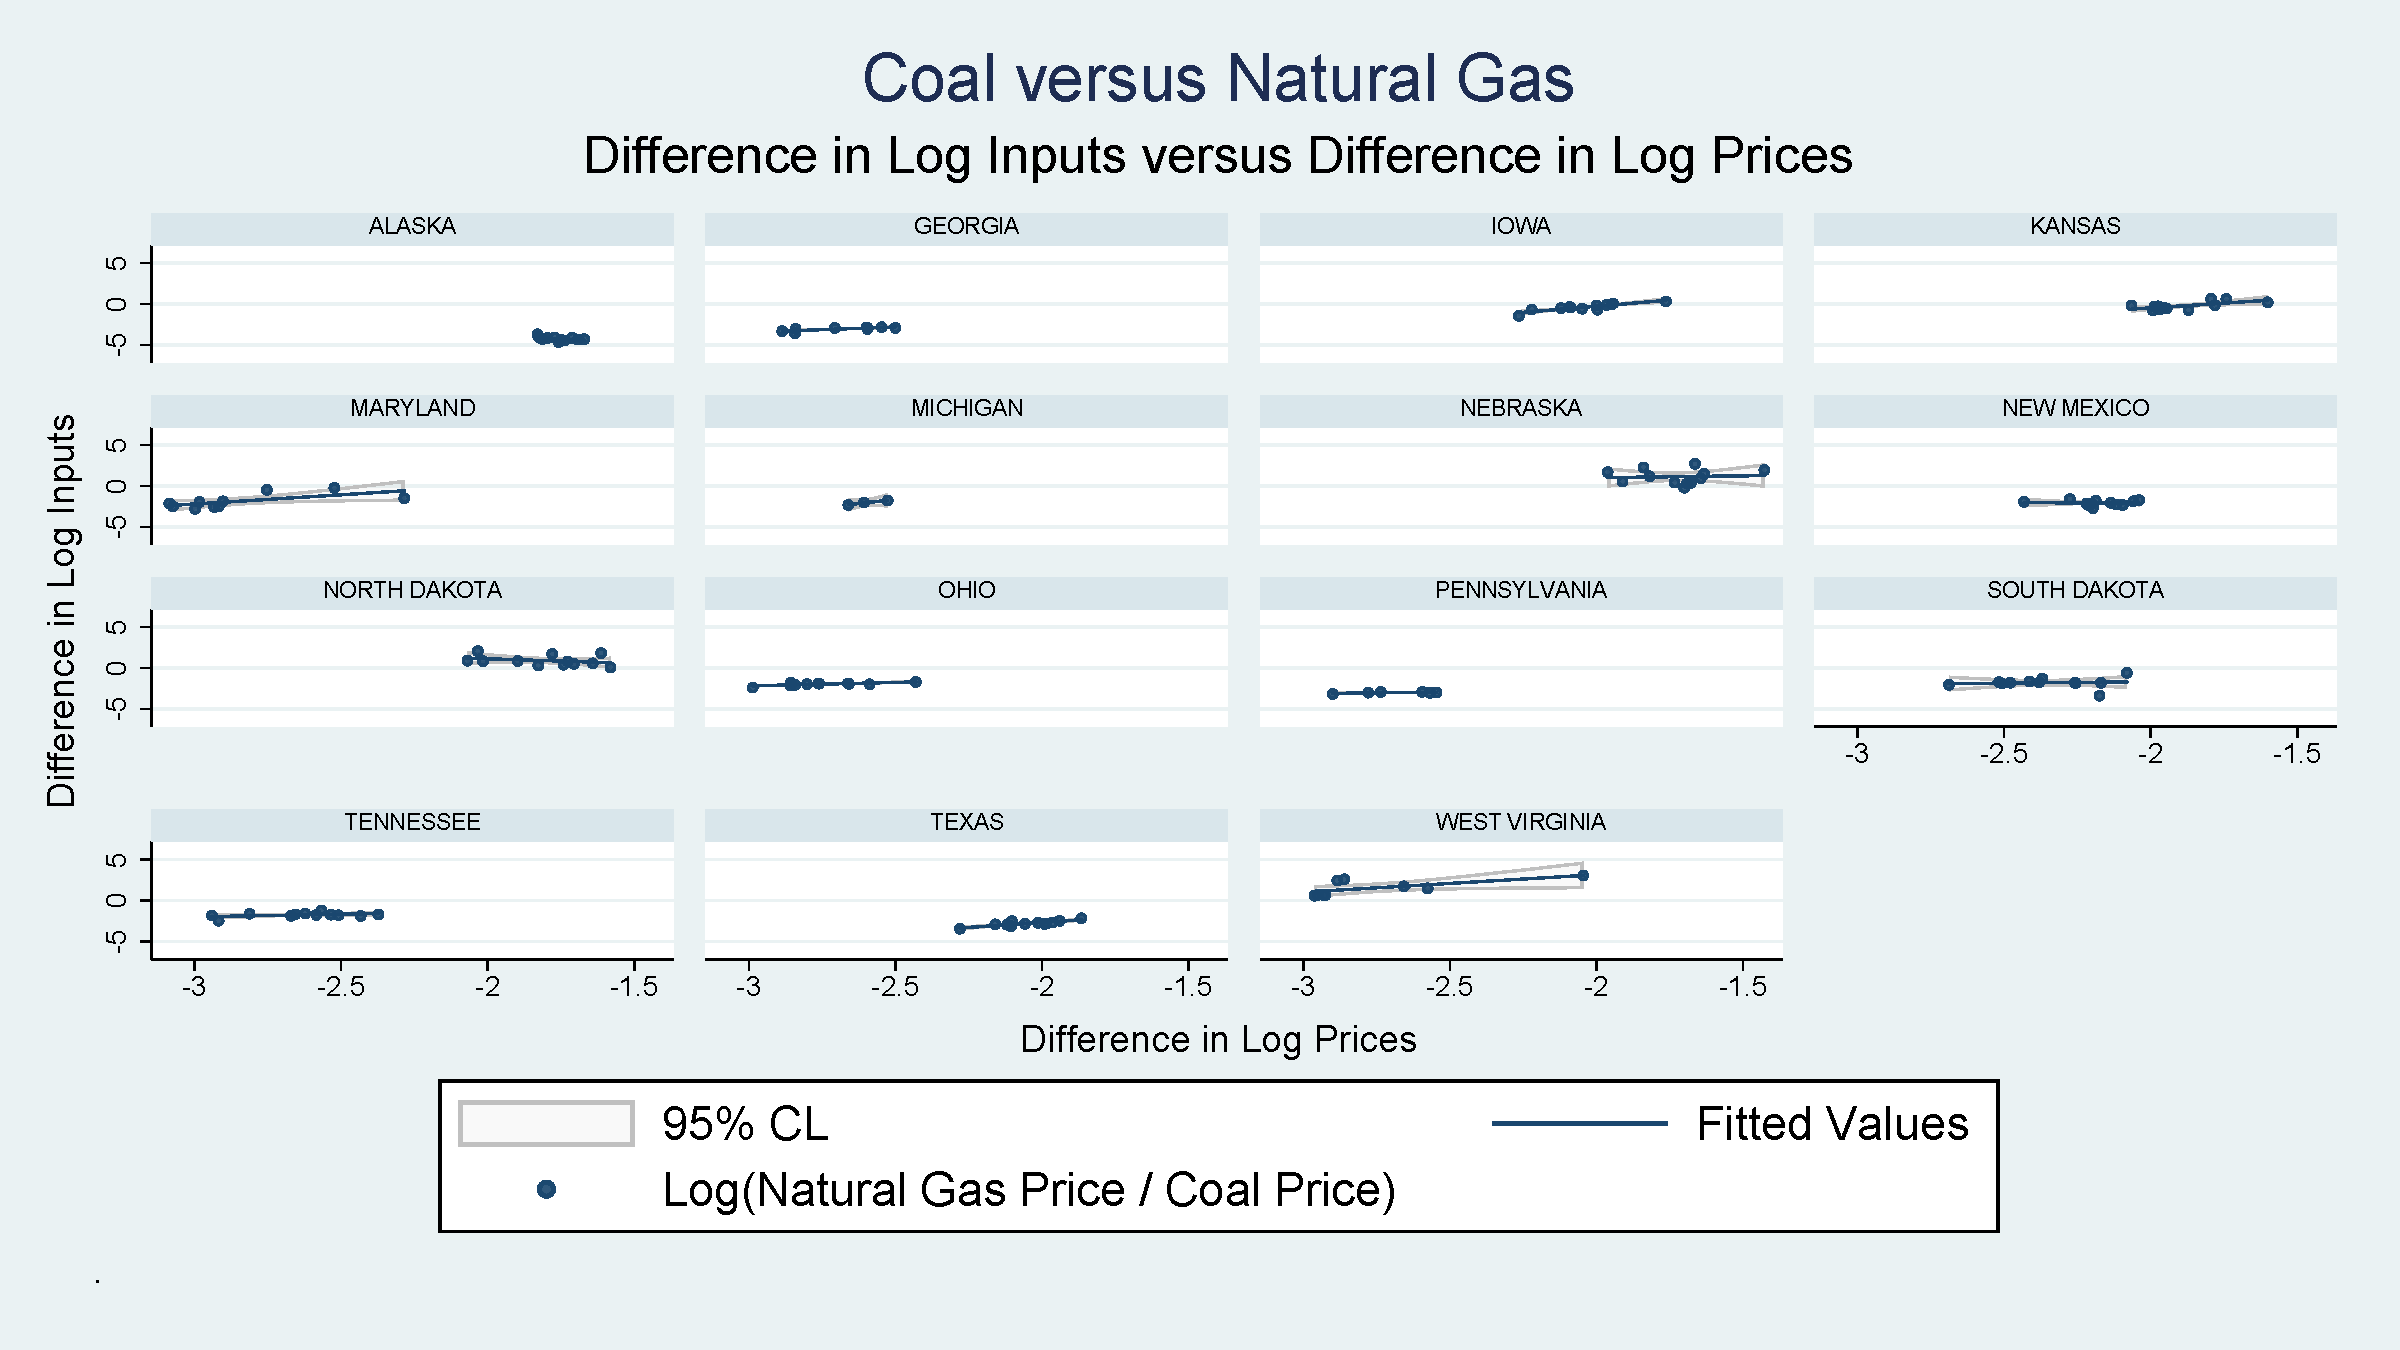
\includegraphics[width=0.9\textwidth]{exhibits/coal_natgas_scatter.pdf} 
\end{center}

\end{frame}


\begin{frame}{Fossil Fuel Results}

\begin{center}
	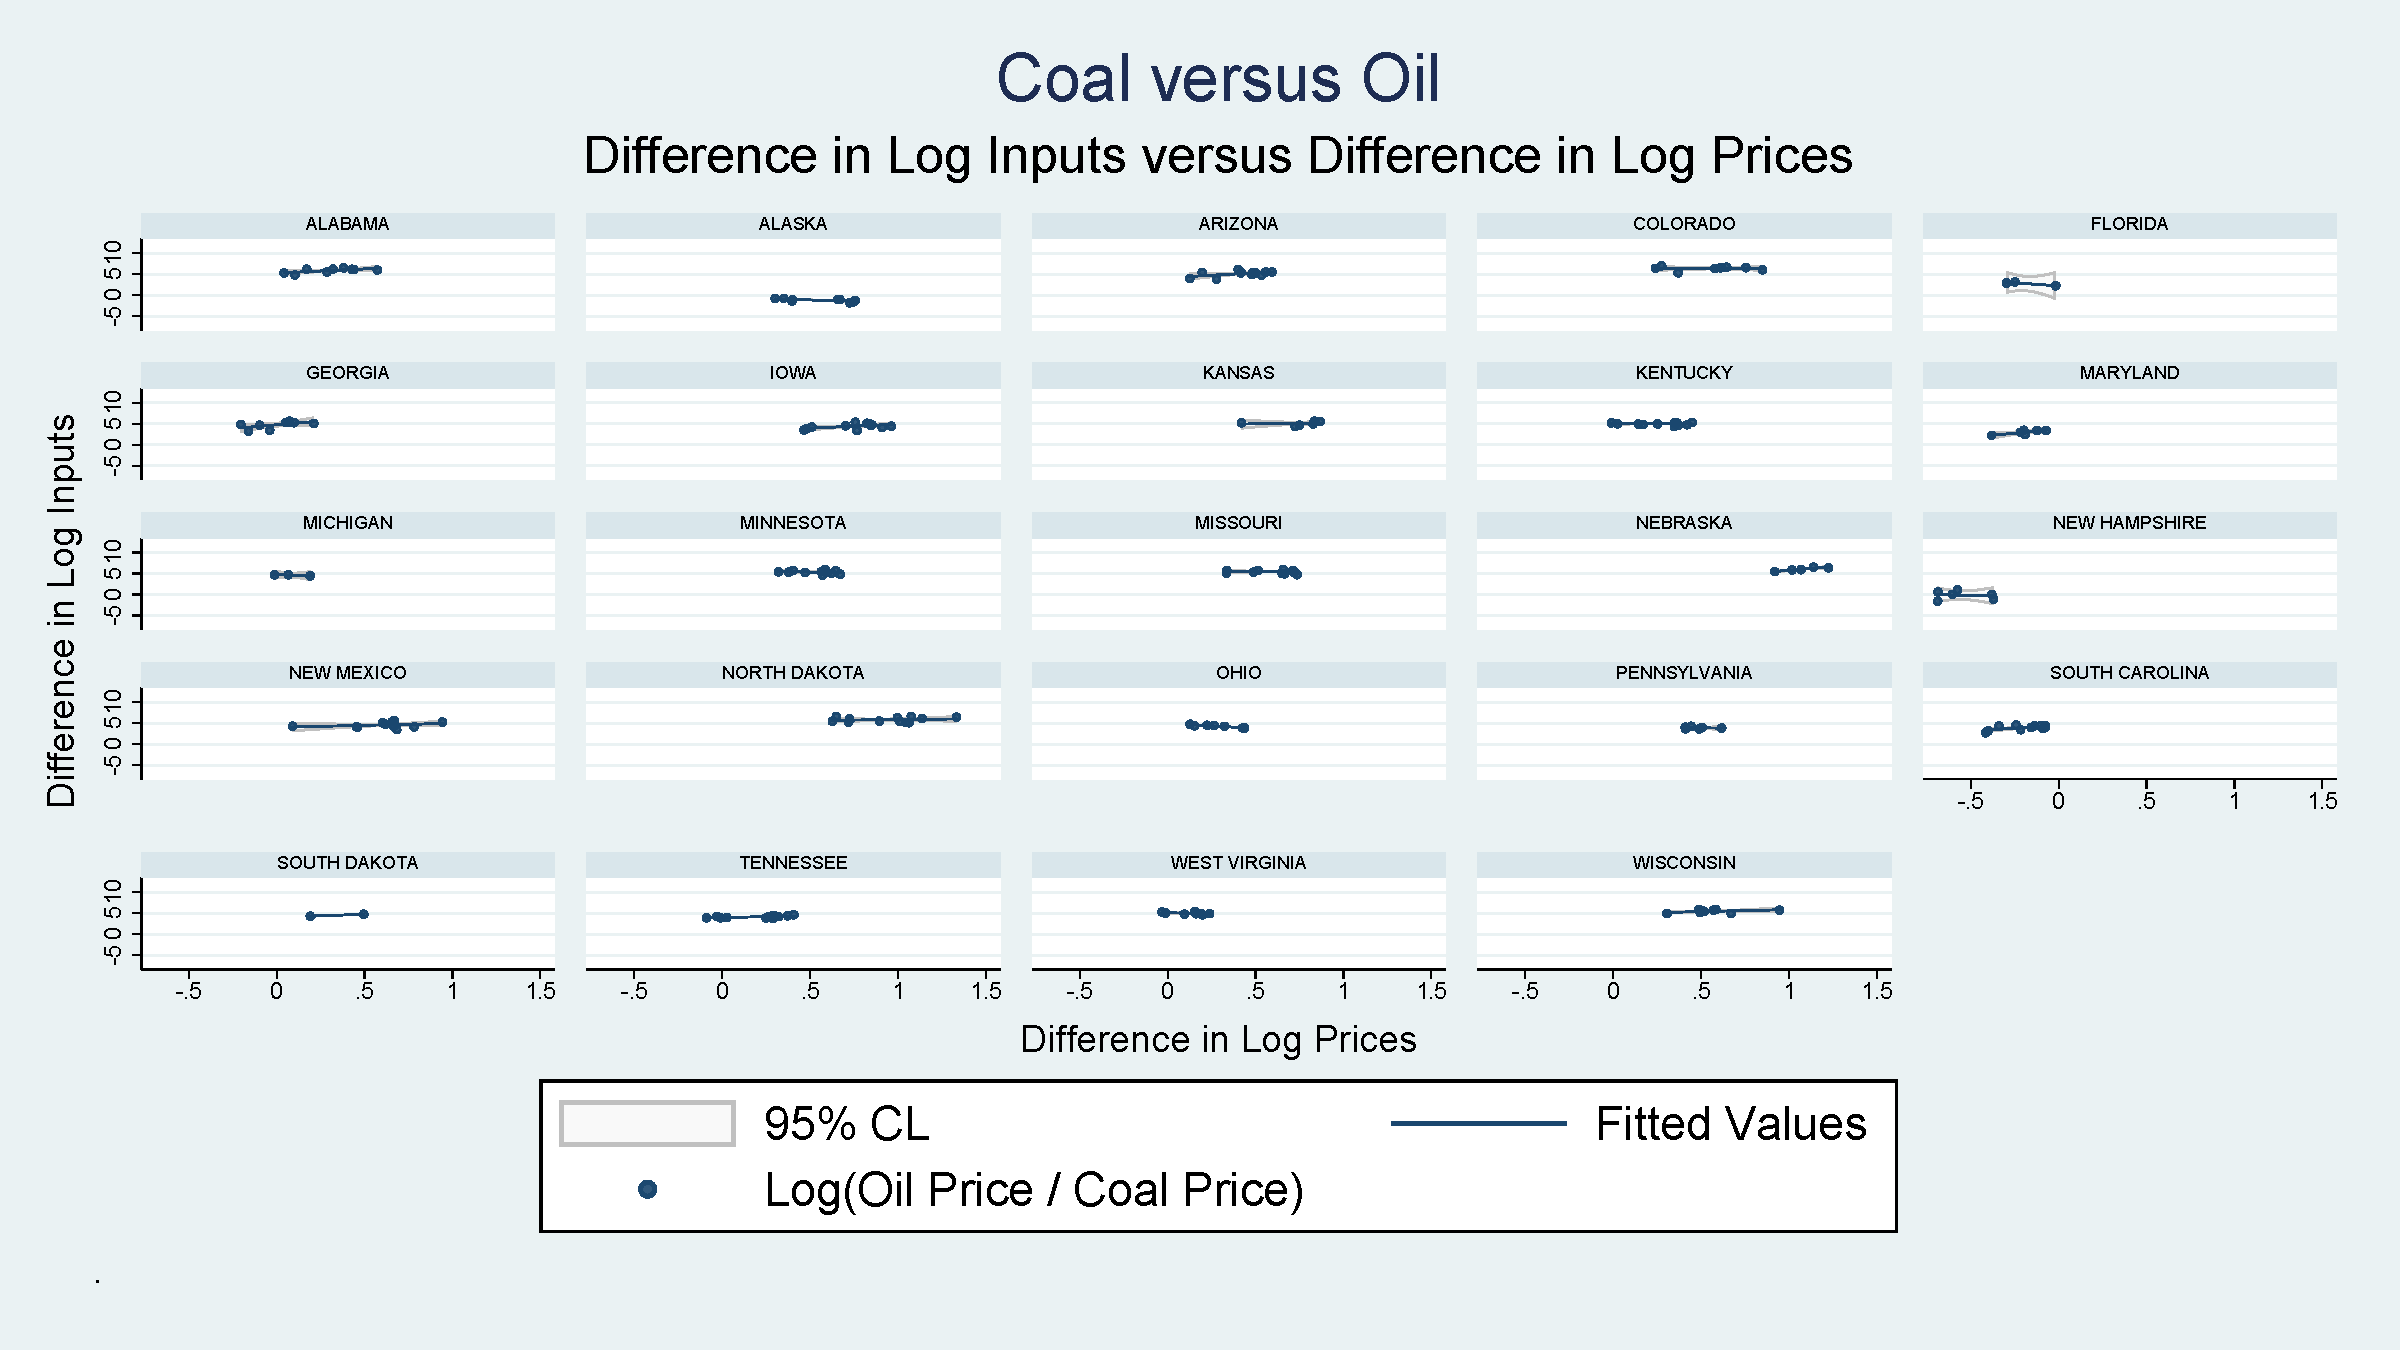
\includegraphics[width=0.9\textwidth]{exhibits/coal_oil_scatter.pdf} 
\end{center}

\end{frame}


\begin{frame}{Fossil Fuel Results}

\begin{center}
	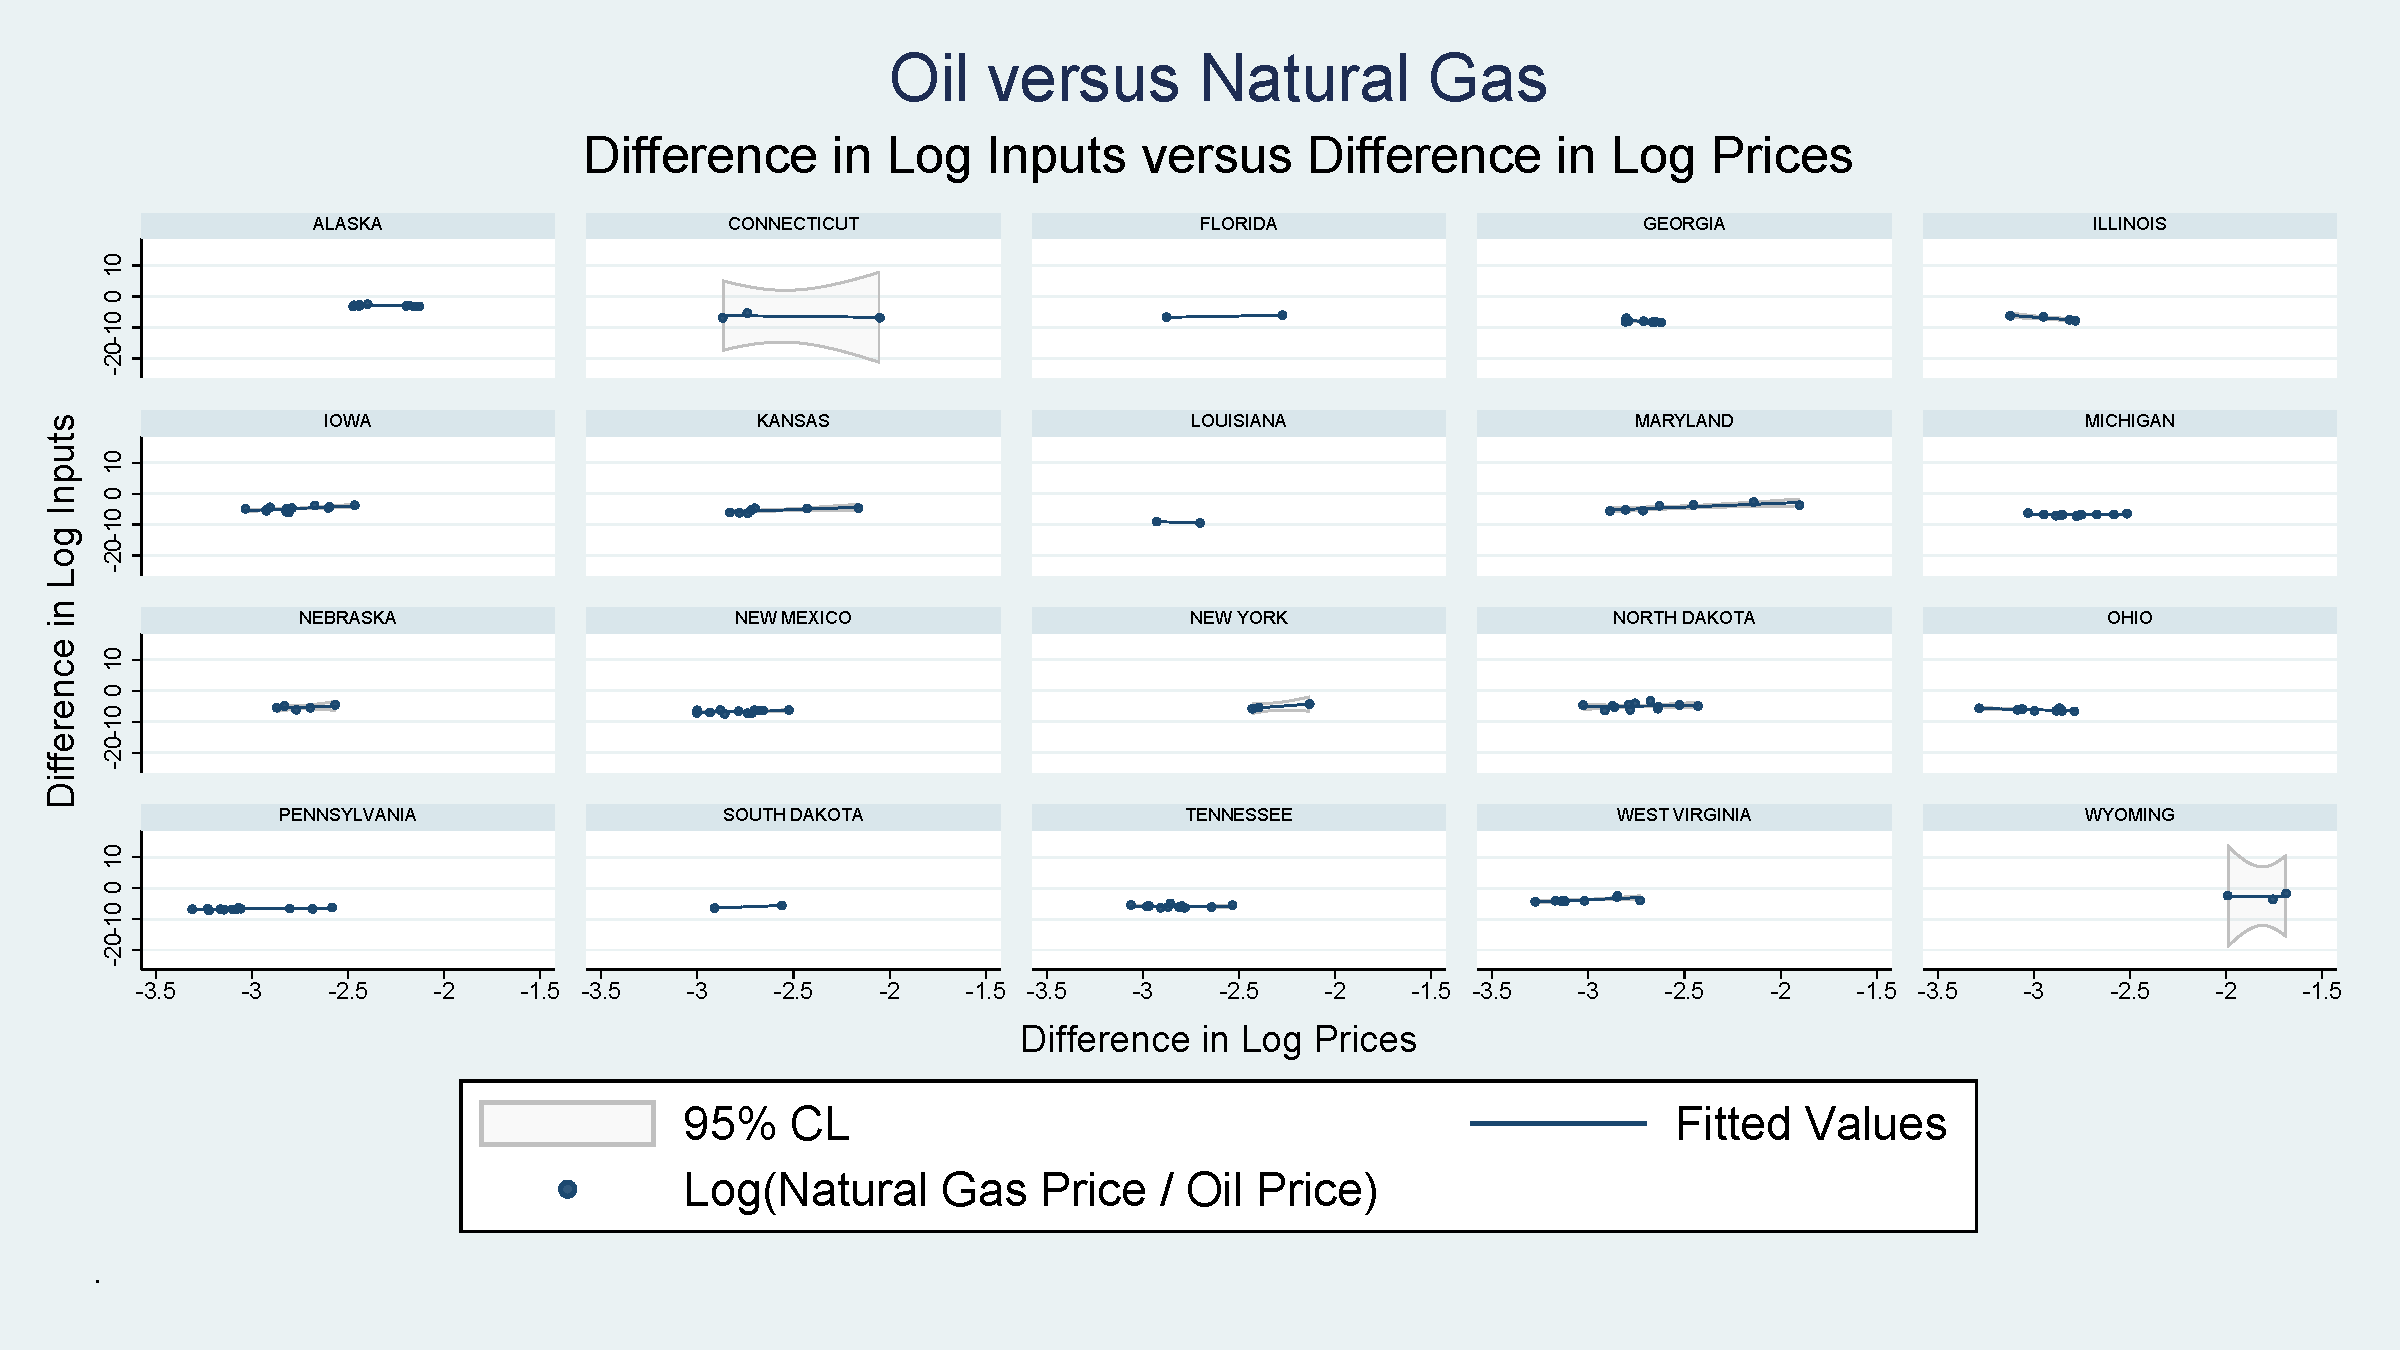
\includegraphics[width=0.9\textwidth]{exhibits/oil_natgas_scatter.pdf} 
\end{center}

\end{frame}



\begin{frame}{Methodology - A Different Approach}

\metroset{block=fill}

\vspace{0.5em}

\begin{block}{\centering{CES Parameter Optimization}}
	$$\min_{\theta, \phi, \alpha, \beta} \; || - \ln \left( Q_{elec} \right) + \ln(\theta) + \frac{1}{\phi} \cdot \ln \left( \alpha_{coal} X_{coal}^\phi + \alpha_{natgas} X_{natgas}^\phi + \alpha_{oil} X_{oil}^\phi\right) + \beta \cdot D_{state} ||_2^2$$
\end{block}

\vspace{-1em}
 
\begin{itemize}
	
	\setlength\itemsep{1em}
	
	\item Can estimate all parameters at once using non-linear least squares 
	
	\item $D_{state}$ represents indicator variables for each state
	
	\item Can also check fit statistics to see if CES functional form matches the data
	
\end{itemize}

\end{frame}


\begin{frame}{Results}

\fontsize{6pt}{7}\selectfont
\begin{center}
	\begin{table}
		\caption{CES Parameter Estimation for Fossil Fuels - NLS} 
		\begin{tabular}{l@{\extracolsep{5em}}cc@{\extracolsep{5em}}c}
			\\[-7ex]\hline  
			\hline \\[-1.2ex]  
			& \multicolumn{3}{c}{\textit{\scriptsize \textit{Dependent Variable}: Electricity Output from Fossil Fuels}} \\ [0.25em] 
			\cline{2-4}  \\[-0.5em] 
			& \multicolumn{3}{c}{$\ln(\theta) + \frac{1}{\phi} \cdot \ln \left( \alpha_{coal} X_{coal}^\phi + \alpha_{natgas} X_{natgas}^\phi + \alpha_{oil} X_{oil}^\phi\right) + \beta \cdot D_{state}$} \\ \\ [-0.7em]
			\hline \\[-1.2ex] 
			$\theta$     &  &       1.144         &       0.676\sym{***}\\
			&&     (0.609)         &    (0.0941)         \\
			[0.5em]
			$\phi$ &   &    \colorbox{yellow}{0.917\sym{***}}&       \colorbox{yellow}{0.900\sym{***}}\\
			&&    (0.0916)         &    (0.0658)         \\
			[0.5em]
			 $\ln(\alpha_{coal})$ &  &     0.533         &       1.147         \\
			&&     (0.433)         &         (.)         \\
			[0.5em]
			$\ln(\alpha_{natgas})$ &&      -1.323\sym{*}  &      -0.925\sym{***}\\
			&&     (0.536)         &     (0.165)         \\
			[0.5em]
			$\ln(\alpha_{oil})$ &   &    1.308         &      -25.94         \\
			&&         (.)         &         (.)         \\ [0.5em]
			State Dummies && \checkmark &   \\ \\ [-0.5em]
			\hline \\ [-0.5em] 
			Observations && 518 & 518  \\ [0.25em]
			R$^2$ & & 0.934   & 0.796    \\  [0.25em]
			Adj. R$^2$ &&  0.928   &  0.795   \\
			\\ [-0.75em] 
			\hline \hline
		\end{tabular} 
	\end{table}
\end{center}



\end{frame}






\begin{frame}{Fossil Fuel Results}

\metroset{block=fill}

\vspace{0.5em}

\begin{block}{\centering{CES $\to$ Cobb-Douglas}}
	$$ \lim_{\phi \to \, 0} \; \theta \cdot \left( \sum_i \; \alpha_i \cdot X_i^\phi \right)^{1/\phi} = \theta \cdot  \prod_i \;  X_i^{\alpha_i} $$
\end{block}

\vspace{-0em}

\begin{itemize}
	
	%\setlength\itemsep{1.5em}
	
	\item Elasticity of substitution ($\sigma = \frac{1}{1-\phi}$) varied by approach
	
	\begin{itemize}
		\item Ratios between commodities led to $\sigma$ around 1 (Cobb-Douglas)
		\item Non-linear least squares led to estimates around 10 (strong substitutes)
	\end{itemize}
	
	
	\item Could try estimating the Translog Function
	
	\begin{itemize}
		\item Second Order Taylor Polynomial of CES around $\phi = 0$
		\item Works best when $\phi \approx 0$ $\implies$ true function is almost Cobb-Douglas
	\end{itemize}
	
	
\end{itemize}


\end{frame}



\begin{frame}{Methodology - Renewables}

	\begin{itemize}
		\setlength\itemsep{1.5em}
		\item Still working on getting production costs for solar and wind
		
		\item Currently have solar and wind elasticities are estimated using 3SLS 
		
		\item Structural Equation Model:
	
		\begin{itemize}
			\item Solar Supply%: Average Solar Radiation, Land Area
			\item Solar Demand%: Population, Cooling/Heating Degree Days
			\item Wind Supply%: Average Wind Speed, Land Area
			\item Wind Demand%: Population, Cooling/Heating Degree Days
		\end{itemize}
		
	\end{itemize}

\end{frame}


\begin{frame}{Methodology - Renewables}

\begin{itemize}
	\item Instrumental Variables Approach
	
	\begin{itemize}
		\item Are price and quantity changes caused by shifts in demand or shifts in supply?
		\item $Q_s = \beta_1 \cdot P + \gamma \cdot Z + \varepsilon_1$
		\item $Q_d = \beta_2 \cdot P + \varepsilon_2$
		\item Z is an instrument in the supply equation $\implies$ identifies the demand curve
		\item Must have $Z$ has independent of demand and good at explaining supply
	\end{itemize}

	\item Instruments for each equation
	
	\begin{itemize}
		\item Solar Supply: Average Solar Radiation, Land Area
		\item Solar Demand: Population, Cooling/Heating Degree Days
		\item Wind Supply: Average Wind Speed, Land Area
		\item Wind Demand: Population, Cooling/Heating Degree Days
	\end{itemize}
	
\end{itemize}

\end{frame}



\begin{frame}{Methodology - Renewables}

\begin{itemize}
	\setlength\itemsep{1.5em}
	
	\item Solar Supply Instruments
	
	\begin{itemize}
		\item Solar energy generation $\approx$ Efficiency $\cdot$ Area $\cdot$ \textbf{Radiation}
		\item Taking logs $\implies$ $\ln(solar\,generation)$ is linear with $\ln(solar\,radiation)$ 
		\item \textbf{Land area} does not seem to have a log-log relationship with $\ln(solar\,generation)$
	\end{itemize}

	\item Solar Demand Instruments

	\begin{itemize}
		\item \textbf{Population} likely multiplicative with solar generation $\implies$ linear function with logs
		\item \textbf{Cooling/Heating Degree Days} - number of degrees that a day's average temperature is below/above room temperature
	\end{itemize}
	
\end{itemize}

\end{frame}


\begin{frame}{Methodology - Renewables}

\begin{itemize}
	\item Wind Supply Instruments
	
	\begin{itemize}
		\item \textbf{Land area} used again here
		\item Wind generation seems to increase exponentially with \textbf{wind speed} in theory
		\item Again, taking logs $\implies \ln(wind\,generation)$ is linear with $(average\,wind\,speed)$
	\end{itemize}

	\begin{center}
		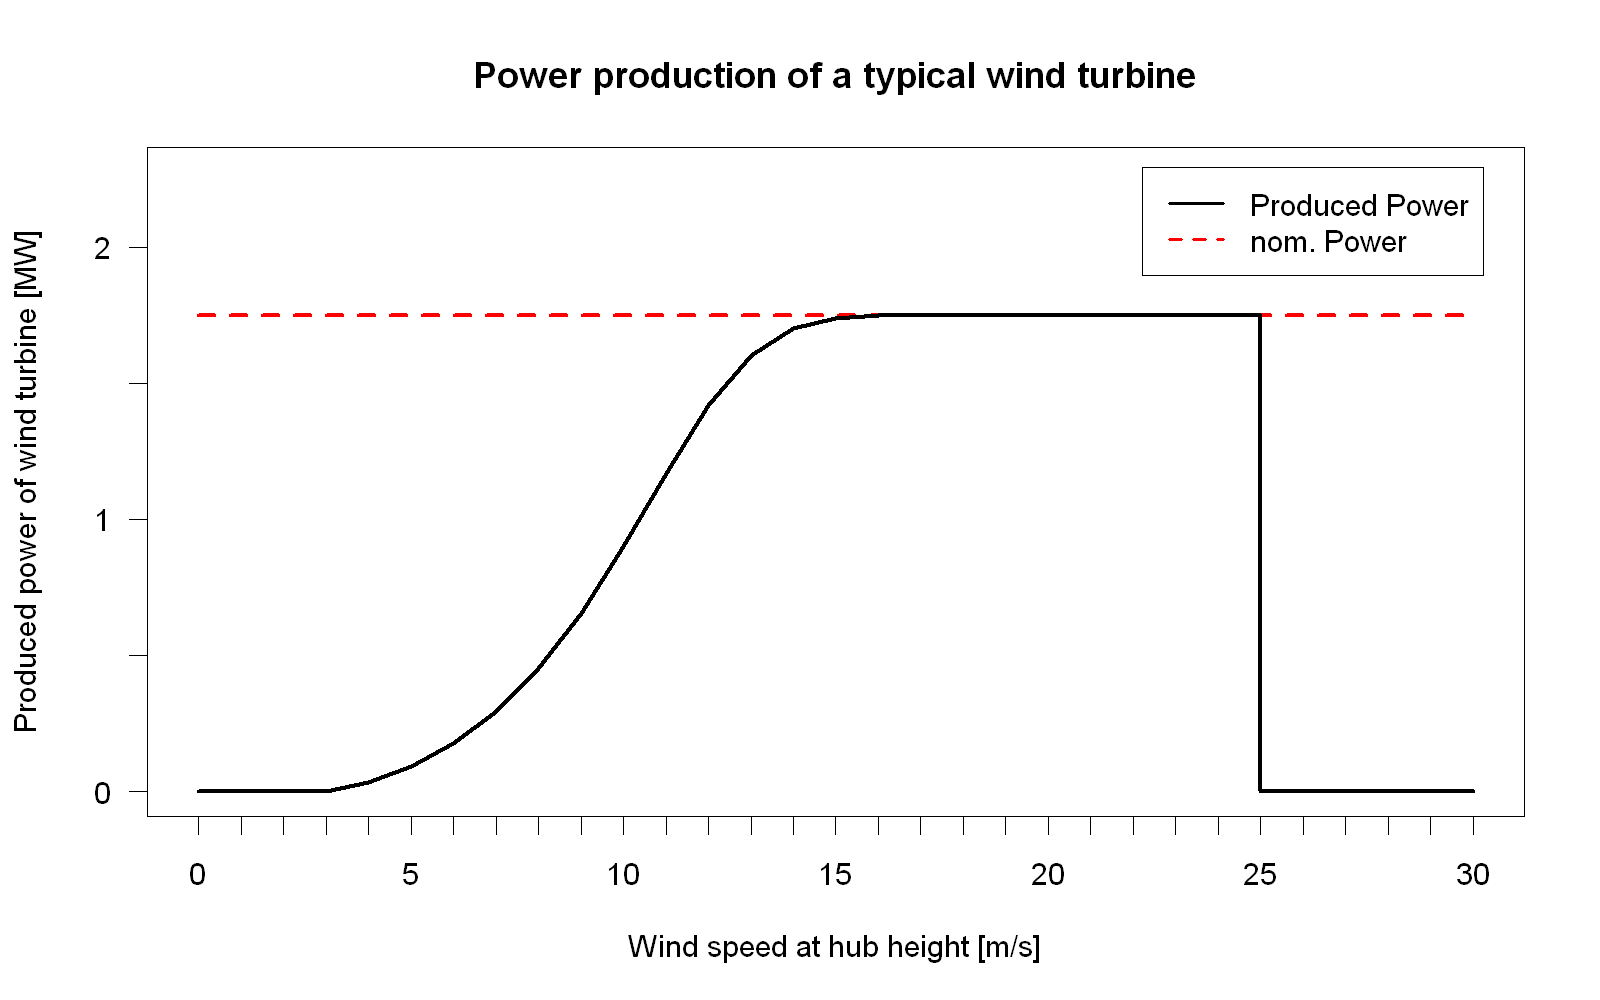
\includegraphics[width=0.4\textwidth]{exhibits/windpowercurve.png} 
	\end{center}
	
	\item Wind Demand Instruments are the same as those for solar
	
\end{itemize}

\end{frame}




\begin{frame}

\fontsize{6pt}{7}\selectfont
\begin{center}
	\begin{table}
		\caption{Elasticities for Solar and Wind - 3SLS Estimation} 
		\begin{tabular}{l*{4}{c}}
			\\[-7ex]\hline  
			\hline \\[-1.2ex]  
			& \multicolumn{4}{c}{\textit{\scriptsize Dependent Variable}} \\ [0.25em] 
			\cline{2-5}  \\[-.5em] 
			& ln(Solar Net Gen) & ln(Solar Net Gen) & ln(Wind Net Gen) & ln(Wind Net Gen) \\ \\ [-0.7em]
			\hline \\[-1.5ex] 
			log(Electricity Price)       &       \colorbox{yellow}{14.46\sym{***}}&     \colorbox{yellow}{ -4.619\sym{*}}  &       \colorbox{yellow}{4.997\sym{***}}&      \colorbox{yellow}{-16.98\sym{***}}\\
			$(cents/kWh)$&     (1.597)         &     (1.911)         &     (1.487)         &     (4.086)         \\
			[0.5em]
			log(Average Solar Radiation)     &       101.5\sym{*}  &                     &                       &                     \\
			$(kWh/m^2)$&     (51.33)         &                     &                     &                     \\
			[0.5em]
			Log(Average Wind Speed)&                     &                     &       0.678\sym{***}&                     \\
			$(m/s)$&                     &                     &    (0.0811)         &                     \\
			[0.5em]
			Land Area    &    1.14e-11\sym{***}&                     &    1.41e-11\sym{***}&                     \\
			$(m^2)$&  (1.16e-12)         &                     &  (9.79e-13)         &                     \\
			[0.5em]
			Log(Population)      &                     &       1.085\sym{***}&                     &       1.166\sym{***}\\
			&                     &     (0.136)         &                     &     (0.286)         \\
			[0.5em]
			Log(Cooling Degree Days)      &                     &      -0.164         &                     &      -0.322         \\
			&                     &     (0.102)         &                     &     (0.191)         \\
			[0.5em]
			Log(Heating Degree Days)      &                     &      -0.169         &                     &     -0.0660         \\
			&                     &     (0.101)         &                     &     (0.182)         \\
			[0.5em]
			Constant      &      -66.97\sym{***}&       7.541         &      -24.11\sym{***}&       65.21\sym{***}\\
			&     (7.367)         &     (7.963)         &     (6.961)         &     (16.81)         \\ \\ [-0.5em] 
			State Dummies &     \checkmark       &    \checkmark     &    \checkmark     &   \checkmark       \\ \\ [-0.5em] 
			\hline \\ [-0.5em] 
			Obs       &         504         &   504                  &            504         &              504       \\
			Chi$^2$        &       109.3$^{***}$         &       81.32$^{***}$         &       76.64$^{***}$         &       41.26$^{***}$         \\\\ [-0.75em] 
			\hline \hline
		\end{tabular}
	\end{table}
\end{center}


]\end{frame}


\begin{frame}{Future Work}

\begin{itemize}
	\setlength\itemsep{1.5em}
	\item Working on non-linear least squares approach for renewables
	
	\item Adding biomass, hydroelectric, nuclear, and geothermal elasticities
	
	\item Elasticity of substitution between clean and dirty energy
	
	\item Can verify final results with price elasticity estimates 
	
\end{itemize}

\end{frame}

\section{Questions?}






\end{document}